\documentclass[letterpaper]{article}

% if you need to pass options to natbib, use, e.g.:
%     \PassOptionsToPackage{numbers, compress}{natbib}
% before loading neurips_2020

% ready for submission
% \usepackage{neurips_2020}

% to compile a preprint version, e.g., for submission to arXiv, add add the
% [preprint] option:
%     \usepackage[preprint]{neurips_2020}

% to compile a camera-ready version, add the [final] option, e.g.:
%     \usepackage[final]{neurips_2020}

% to avoid loading the natbib package, add option nonatbib:
\usepackage[nonatbib]{neurips_2020}

\usepackage[utf8]{inputenc} % allow utf-8 input
\usepackage[T1]{fontenc}    % use 8-bit T1 fonts
\usepackage{hyperref}       % hyperlinks
\usepackage{url}            % simple URL typesetting
\usepackage{booktabs}       % professional-quality tables
\usepackage{amsfonts}       % blackboard math symbols
\usepackage{nicefrac}       % compact symbols for 1/2, etc.
\usepackage{microtype}      % microtypography
\usepackage{amssymb}
\usepackage{amsmath}
\usepackage{amsfonts}
\usepackage{algorithm}
\usepackage{algpseudocode}
\usepackage{bbm}
\usepackage{graphicx}
\usepackage{mwe}
\usepackage{caption}
\usepackage{subcaption}

\newcommand{\setN}{\mathbb{N}} % natuerliche Zahlen
\newcommand{\setZ}{\mathbb{Z}} % ganze Zahlen
\newcommand{\setQ}{\mathbb{Q}} % gebrochene Zahlen
\newcommand{\setR}{\mathbb{R}} % reelle Zahlen
\newcommand{\setC}{\mathbb{C}} % komplexe Zahlen
\newcommand{\setId}{\mathbb{I}} % Id
\newcommand{\kA}{\mathcal{A}}   %kaligraphisches A
\newcommand{\kC}{\mathcal{C}}   %kaligraphisches C
\newcommand{\kD}{\mathcal{D}}   %kaligraphisches D
\newcommand{\kI}{\mathcal{I}}   %kaligraphisches I
\newcommand{\kJ}{\mathcal{J}}   %kaligraphisches J
\newcommand{\kT}{\mathcal{T}}   %kaligraphisches T
\newcommand{\kE}{\mathcal{E}}   %kaligraphisches E
\newcommand{\kF}{\mathcal{F}}   %kaligraphisches F
\newcommand{\kG}{\mathcal{G}}   %kaligraphisches G
\newcommand{\kK}{\mathcal{K}}   %kaligraphisches K
\newcommand{\kH}{\mathcal{H}}   %kaligraphisches H
\newcommand{\kL}{\mathcal{L}}   %kaligraphisches L
\newcommand{\kM}{\mathcal{M}}   %kaligraphisches M
\newcommand{\kN}{\mathcal{N}}   %kaligraphisches N
\newcommand{\kS}{\mathcal{S}}   %kaligraphisches S
\newcommand{\kP}{\mathcal{P}}   %kaligraphisches P
\newcommand{\kX}{\mathcal{X}}   %kaligraphisches X
\newcommand{\kY}{\mathcal{Y}}   %kaligraphisches Y
\newcommand{\Ind}{\mathbbm{1}} % Ind
\newcommand{\code}[1]{\texttt{#1}}

% Mathematical Environments
\newtheorem{Ax}{Axiom}
\newtheorem{Def}{Definition}
\newtheorem{Bsp}{Example}
\newtheorem{Bem}{Remark}
\newtheorem{Satz}{Proposition}
\newtheorem{HSatz}{Theorem}
\newtheorem{Lemma}{Lemma}
\newtheorem{Korollar}{Corollary}
\newenvironment{Proof}{\par {\it Proof.} \par}{\hspace*{\fill}
$\Box$\par\vskip2ex}    %Beweisumgebung


\newcommand{\vol}{{\rm vol}}
\newcommand{\diag}{{\rm diag}}
\newcommand{\tr}{{\rm tr}}
\newcommand{\sgn}{{\rm sgn}}
\newcommand{\DO}{{\rm do}}
\newcommand{\supp}{{\rm supp}}
\newcommand{\PN}{{\rm PN}}
\newcommand{\PS}{{\rm PS}}
\newcommand{\PNS}{{\rm PNS}}

\newcommand{\diff}{{\rm Diff}}
\newcommand{\pa}{{\rm pa}}
\newcommand{\de}{{\rm de}}
\newcommand{\nei}{{\rm ne}}
\newcommand{\ch}{{\rm ch}}
\newcommand{\nd}{{\rm nd}}
\newcommand{\an}{{\rm an}}
\newcommand{\An}{{\rm An}}
\newcommand{\bd}{{\rm bd}}
\newcommand{\cl}{{\rm cl}}
\setcounter{MaxMatrixCols}{17}

\renewcommand{\algorithmicrequire}{\textbf{Input:}}
\renewcommand{\algorithmicensure}{\textbf{Output:}}

\title{Information-Theoretic Approximation to Causal Models}

% The \author macro works with any number of authors. There are two commands
% used to separate the names and addresses of multiple authors: \And and \AND.
%
% Using \And between authors leaves it to LaTeX to determine where to break the
% lines. Using \AND forces a line break at that point. So, if LaTeX puts 3 of 4
% authors names on the first line, and the last on the second line, try using
% \AND instead of \And before the third author name.

\author{%
  Peter Gmeiner \\
  Global Data Science\\
  GfK SE, Germany\\
  \texttt{peter.gmeiner@gfk.com} \\
  % examples of more authors
  % \And
  % Coauthor \\
  % Affiliation \\
  % Address \\
  % \texttt{email} \\
  % \AND
  % Coauthor \\
  % Affiliation \\
  % Address \\
  % \texttt{email} \\
  % \And
  % Coauthor \\
  % Affiliation \\
  % Address \\
  % \texttt{email} \\
  % \And
  % Coauthor \\
  % Affiliation \\
  % Address \\
  % \texttt{email} \\
}

\begin{document}

\maketitle

\begin{abstract}
Inferring the causal direction and causal effect between two discrete random variables $X$ and $Y$ from a finite sample is often a crucial problem and a challenging task. However, if we have access to observational and interventional data, it is possible to solve that task. If $X$ is causing $Y$, then it does not matter if we observe an effect in $Y$ by observing changes in $X$ or by intervening actively on $X$. This invariance principle creates a link between observational and interventional distributions in a higher dimensional probability space. We embed distributions that originate from samples of $X$ and $Y$ into that higher dimensional space such that the embedded distribution is closest to the distributions that follow the invariance principle, with respect to the relative entropy. This allows us to calculate the best information-theoretic approximation for a given empirical distribution, that follows an assumed underlying causal model. We show that this information-theoretic approximation to causal models (IACM) can be done by solving a linear optimization problem. In particular, by approximating the empirical distribution to a monotonic causal model, we can calculate probabilities of causation. It turns out that this approximation approach can be used to successfully solve causal discovery problems in the bivariate, discrete case. Experimental results on both labeled synthetic and real-world data demonstrate that our approach outperforms other state-of-the-art approaches in the discrete case with low cardinality.
\end{abstract}

\section{Introduction}

Detecting causal relationships from data is a major issue in many disciplines. The understanding of causal relations between variables can help to understand how a system behaves under intervention, stabilize future predictions, and has many other important implications. Identifying causal relations (causal discovery) from observed data alone is only possible with further assumptions and/or additional data. Pearl proposed in  \cite{Pea09} a mathematical framework that formalizes causality and causal relations. This framework allows a systematic study of causal models and their identification. That are models that represent an (unknown) underlying data generation mechanism that is responsible for the distribution of the sampled data \cite{PJS17}. Despite the various causal discovery methods available the problem of finding the causal structure of random variables is still not sufficiently solved. In particular, the case with two random variables $X$ and $Y$ remains challenging and some methods fail to resolve the causal direction in that case. However, under certain assumptions, we can infer the correct causal direction. One example is to include sampled data from situations (environments) where interventions took place together with samples from observations. Recent developments in that direction revealed promising results \cite{PBM16, HPM18}, but often these methods are conservative leading to situations were no direction is preferred. This paper focuses on the bivariate discrete case and is based on a natural and weak principle. The principle of independent mechanism assumes that the data generating mechanism is independent of the data that is feed into such a mechanism. From this principle, we derive an invariance relation that states that it does not matter if we observe an effect due to an observation of its cause or due to an intervention on its cause. Distributions that are generated by an underlying causal model fulfill these invariance relations. If $X$ and $Y$ are discrete random variables, then we can characterize the set of joint distributions that fulfill these relations by embedding them into a higher-dimensional space. This allows us to link distributions from observational and interventional samples and embed them into that higher-dimensional space. That means we first embed the empirical distributions into a higher-dimensional space and then find the best approximation of this embedding to the probability distributions that are compatible with the invariance principle such that the relative entropy between them is minimized. We call this approach an information-theoretic approximation to causal models (IACM). The relative entropy can be interpreted as an error that tells us how much a finite sample deviates from a sample that comes from an assumed underlying causal model. It turns out that solving this optimization problem is equivalent to solving a linear optimization problem which ends up in an efficient algorithm.

With respective preprocessing we can apply IACM also to continuous data. This allows us to formulate a causal discovery algorithm that infers the causal direction of two random variables. For this, we apply the approximation to a causal model were $X$ causes $Y$ and to a model were $Y$ causes $X$. We prefer the direction that has lower relative entropy.

If we additionally assume that the underlying causal model is monotonic w.r.t. $X$ or $Y$, then we can include this assumption into our approach. For binary random variables, Pearl defined counterfactual statements that give information about how necessary, sufficient, or necessary and sufficient a cause is for an effect \cite{Pea09}. If the variables are generated by a monotonic causal model he also provides closed formulas for these measures. We can use this as a strength of a causal link by using the approximated distribution to a monotonic causal model. We also include the approximation to that more specific model into our causal discovery algorithm.

The contribution of this paper is twofold. Let us assume that we have two random variables $X$ and $Y$ that attain values in finite ranges $\kX_X$ and $\kX_Y$, respectively. If we know (or assume) for some reason the causal direction and have data from $X, Y$ available that come from observations and experiments, then our first contribution is a new method for approximating empirical probability distributions such that they fulfill an invariance condition of the assumed causal model. With sophisticated preprocessing, this method can even then be applied if we only know that the data are heterogeneous. If we further assume monotonicity, then we can calculate probability measures for the assumed causal relation. The second contribution is a method for causal discovery that is based on this approximation procedure. By measuring the distance between the empirical probability distribution and its causal model approximation we can formulate a simple causal discovery algorithm. This causal discovery algorithm can also be applied if we have observed data from $X$ and $Y$ that are heterogeneous and continuous. In experiments, we were able to verify the strength of our causal discovery approach in the case that we have discrete ranges with low cardinality. For that case, we outperformed alternative state of the art methods.

The paper is organized as follows. Section \ref{sec.causalModels} introduces causal models and formulates the invariance statement. In Section \ref{sec.iacm} we present an information-theoretic
approximation of distributions to one that is generated by causal models. We derive the theoretic foundation for the general case, illustrate the results for the binary case, and formulate the approximation algorithm. Section \ref{sec.applications} shows some applications of the approximation algorithm. In particular, we discuss the calculation of probabilities for causes, the application to timeseries data, and the application to causal discovery. Section \ref{sec.experiments} describes experiments to verify the approach and Section \ref{sec.discussion} concludes with a discussion.

\section{Causal Models} \label{sec.causalModels}

In this section we introduce models to formally describe causality and causal relations. We describe causal relations in the form of a {\em directed graph} $G=(V,E)$ with a finite vertex set $V$ and a set of directed edges $E \subset V \times V$. A {\em directed edge} from $u \in V$ to $v \in V$ is an ordered pair $(u,v)$ and often represented as an arrow between vertices, e.g. $u \rightarrow v$. For a directed edge $(u,v)$ the vertex $u$ is a {\em parent} of $v$ and $v$ is a {\em child} of $u$. The set of parents of a vertex $u$ is denoted by ${\rm PA}_u$. In this paper we only consider directed graphs that have no cycles and call them directed acyclic graphs (DAGs). In a DAG we interpret the vertices as random variables $V=\{X_1, \ldots, X_n\}$ and a directed edge $(X_i, X_j)$ as a causal link between $X_i$ and $X_j$. We say that $X_i$ is a {\em direct cause} of $X_j$ and $X_j$ is a {\em direct effect} of $X_i$. We can further specify those causal links by introducing functional relations between parent and child vertices.

\begin{Def}
A {\bf structural causal model} (SCM) is a tuple $\kC:=(S, P_N)$ where $S$ is a collection of $L$ structural assignments
$$
X_j:=f_j ({\rm PA}_j, N_j), \qquad j=1, \ldots, L,
$$
where ${\rm PA}_j \subseteq \{X_1, \ldots, X_L\} \backslash \{X_j\}$ are the parents of $X_j$ and $P_N = P_{N_1, \ldots, N_L}$ is a joint distribution over the noise variables $N_j$ that are assumed to be jointly independent.
\end{Def}

We consider an SCM as a model for a data-generating process \cite{PJS17}. This enables us to model a system in an observational state and under perturbations at the same time. An SCM defines a unique distribution $P^{\kC}_X$ over the variables $X=(X_1, \ldots, X_d)$. Perfect {\em interventions} can be formalized by replacing an assignment in an SCM. Given an SCM $\kC$ we can replace the assignment for $X_k$ by $X_k := \tilde f(\tilde{{\rm PA}}_k, \tilde N_k)$. The distribution of that new SCM $\tilde \kC$ is denoted by $P_X^{\tilde \kC} =: P_X^{\kC; \DO(X_k:=\tilde f(\tilde{{\rm PA}}_k, \tilde N_k))}$ and called {\em intervention distribution} \cite{PJS17, Pea09}.

When modeling causality we assume the {\em principle of independent mechanism}. Roughly speaking this principle states that a change in a variable does not change the underlying causal mechanism, see \cite{PJS17}. Formally for an SCM, this would mean that a change in a child variable $X$ will not change the mechanism $f$ that is responsible to obtain an effect from $X$. From this principle the following invariance statement follows:

\begin{equation} \label{consistencyCondition}
p^\kC(x_j | x_{{\rm PA}_j}) = p^{\kC; \DO(X_k:=x)}(x_j|x_{{\rm PA}_j}),
\end{equation}
where $p(x_j|x_{{\rm PA}_j})$ is the conditional density of $P_{X_j|X_{{\rm PA}_j}=x_{{\rm PA}_j}}$ evaluated at $x_j$ for some $k \neq j$. Informally, this condition means that if there is a cause $X_k$ which has $X_j$ as an effect, then it doesn't matter if we observe $x_j$ when $x$ is present or if we observe $x_j$ when $x$ is present due to an intervention on $X_k$. 

\section{Approximation to Causal Models} \label{sec.iacm}

\subsection{The General Case} \label{section.general_case}

Given two random variables $X, Y$ with finite ranges $\kX_X, \kX_Y$, and data from observations of $X, Y$ as well as from interventions on $X$ or $Y$. We can also relax that assumption and assume instead that the data are heterogeneous and show a rich diversity. Formally we have observed data of $X$ and $Y$ and data from perfect interventions on $X$ or $Y$ denoted as $X_a, Y_a$ when the intervention on $X$ or $Y$ was some $a \in \kX_X$ or $a \in \kX_Y$, respectively.\footnote{Alternatively, we can say that we have data of $X$ and $Y$ from different environments, where each environment belongs to a different intervention on $X$ or $Y$.} We further assume that the different interventional data are independent of each other. In practical applications, these interventional data can be obtained from experiments or more implicit from heterogeneous data.

Condition (\ref{consistencyCondition}) is in general not fulfilled by empirical distributions that are obtained from such data. In this section, we derive a method that enables us to find a joint probability distribution of $X$ and $Y$ that fulfill the consistency condition (\ref{consistencyCondition}) and is closest to a given empirical distribution in an information-theoretic sense.

Without loss of generality we assume that the intervention took place on $X$ with values in $\kX_X=\{x_1, \ldots, x_d\}$, where $d:= |\kX_X|$. We summarize ${\bf X}:= (X, (X_a)_{a \in \kX_X})$, ${\bf Y}:=(Y,(Y_a)_{a \in \kX_X})$, where $X,Y$ are the observed data and $(X_a)_{a \in \kX_X}, (Y_a)_{a \in \kX_X}$ the interventional data. We define $V:=\{X, Y, Y_{x_1}, \ldots, Y_{x_d}\}$ that takes values in $\kX_V:=\kX_X \times \kX_Y \times \kX_{Y_{x_1}} \times \ldots \times \kX_{Y_{x_d}}$ and with $P_{V}$ we denote the joint distribution over $V$. The space of probability distributions on $\kX_V$ is denoted by $\kP(\kX_V)$ and for $A \subset V$ the marginalization of a probability distribution $P \in \kP(\kX_V)$ is defined by $\pi_A : \kP(\kX_V) \rightarrow \kP(\kX_A)$ with $\pi_A(P)(x):= \sum_{y\in \kX_{V \backslash A}} P(y,x)$, where $x\in \kX_A$ and $\kX_A := \times_{a \in A} \kX_a$. The next Lemma give us a characterization of distributions that fulfill condition (\ref{consistencyCondition}).

\begin{Lemma}
The set of joint probability distributions for $X, Y, Y_{x_1}, \ldots, Y_{x_d}$ which fulfill the consistency condition (\ref{consistencyCondition}) is called $\kM_C$ and given as
\begin{eqnarray*}
\kM_C & = & \left \{P \in \kP(\kX_V) \mid \pi_{X, Y, Y_{x_i}} P(x_i, y, \overline{y}_{x_i}) = \pi_{X, Y, Y_{x_i}} P(x_i, \overline{y}, y_{x_i}) = 0 \right. \\
& & \qquad \qquad \qquad \left. \forall \; y \in \kX_Y, y_{x_i} \in \kX_{Y_{x_i}}, i \in \{1, \ldots, d\} \right \},
\end{eqnarray*}
where $\overline{y}_{x_i} \in \kX_{Y_{x_i}} \backslash \{y_{x_i}\}$ for $i \in \{1, \ldots, d\}$ and $\overline{y} \in \kX_Y \backslash \{y\}$.
\end{Lemma}
\begin{Proof}
The consistency condition (\ref{consistencyCondition}) implies the following relation for some $P \in \kP(\kX_V)$ and $i\in \{1,\ldots, d\}$
\begin{eqnarray*}
\pi_{X, Y} P(x_i, y) & = & \pi_{X, Y, Y_{x_i}} P(x_i, y, y_{x_i}), \qquad {\rm with} \; y=y_{x_i}.
\end{eqnarray*}
These relation implies
\begin{eqnarray*}
\pi_{X, Y, Y_{x_i}} P(x_i, y, \overline{y}_{x_i}) = \pi_{X, Y, Y_{x_i}} P(x_i, \overline{y}, y_{x_i}) = 0, {\rm \;for}\;i \in\{1,\ldots, d\},
\end{eqnarray*}
which characterizes the joint distributions that satisfy (\ref{consistencyCondition}).
\end{Proof}

The support of $\kM_C$ is therefore given by 
\begin{eqnarray*}
\supp(\kM_C) = \left \{\kX_V \backslash \! \! \! \! \! \! \bigcup_{\stackrel{y\in\kX_Y, y_{x_i}\in \kX_{Y_{x_i}},y=y_{x_i},}{x_i \in \kX_X, i\in \{1,\ldots, d\}}} \! \! \! \! \! \! \! \! \! x_i \times y \times \kX_{Y_{x_1}} \times \ldots \times \kX_{Y_{x_{i-1}}} \times y_{x_i} \times \kX_{Y_{x_{i+1}}} \times \ldots \times \kX_{Y_{x_d}} \right \}.
\end{eqnarray*}

Given observation and intervention data of $X$ and $Y$ and its corresponding empirical distributions $P_{X,Y}$, $P_{Y_{x_i}}$ for $i \in \{1,\ldots, d\}$ we try to find a distribution $\hat P \in \kM_C$ such that
\begin{equation} \label{equ.marginalization_problem}
\pi_{X,Y} \hat P = P_{X,Y}, \quad {\rm and}\; \pi_{Y_{x_i}} \hat P = P_{Y_{x_i}} \; {\rm for} \; x_i \in \kX_X, i\in \{1, \ldots, d\}.
\end{equation}

We can always find a joint distribution $\hat P \in \kP(\kX_V)$ such that (\ref{equ.marginalization_problem}) holds, since  the distributions $P_{XY}, P_{Y_{x_i}}$ for all $x_i \in \kX_X$ are independent to each other. But this does not guarantee that $\hat P \in \kM_C$. Nevertheless, we can try to find a distribution in $\kM_C$ that has minimal relative entropy to $\hat P$.\footnote{In other words we try to find the information-geometric projection of $\hat P$ to $\kM_C$.} This minimal relative entropy can be interpreted as an approximation error to the assumed causal model. The {\em relative entropy} or {\em Kullback-Leibler divergence} (KL-divergence) between two distributions $P, Q \in \kP(\kX_V)$ is defined as follows
$$
D(P || Q) := \left \{ \begin{array}{ll}
\sum_{x \in \kX_V} P(x) \log \left (\frac{P(x)}{Q(x)}\right ), & {\rm if\;} \supp(Q) \supseteq \supp(P), \\
\infty, & {\rm else.}
\end{array}
\right.
$$
We use the convention that $0 \log \frac{0}{q} = 0$ for $q > 0$. The relative entropy is not symmetric, but it holds that $D(P||Q) \ge 0$, with equality if and only if $P=Q$. Although, it is not a distance measure it is an important quantity that appears in many contexts concerning information and probability theory, see \cite{CT91, Kak99}. 

This lead us to the following optimization problem:

\begin{equation} \label{equ.MinMinProblem}
\min_{\substack{\hat P \in \kP(\kX_V),\\ \pi_{X,Y} \hat P = P_{XY}, \pi_{Y_{x_i}} \hat P = P_{Y_{x_i}}}} \min_{\tilde P \in \kM_C} D(\hat P|| \tilde P).
\end{equation}
This is a nonlinear min-min optimization problem with linear constraints. But it turns out that in our situation the problem simplifies to a linear optimization problem.

\begin{Satz} \label{prop.approx_solution}
The optimization problem (\ref{equ.MinMinProblem}) simplifies to the following linear optimization problem
$$
\max_{\substack{\hat P \in \kP(\kX_V),\\ \pi_{X,Y} \hat P = P_{XY}, \pi_{Y_{x_i}} \hat P = P_{Y_{x_i}}}} S(\hat P),
$$
with $S(\hat P):= \sum_{z \in \supp(\kM_C)} \hat P(z)$.
\end{Satz}
\begin{Proof}
We first consider the inner minimization problem of (\ref{equ.MinMinProblem}) for a given joint distribution $\hat P \in \kP(\kX_V)$. This is a constrained optimization problem where the constraints in $\kM_C$ are equivalent to the equation
$$
S(\tilde P) = 1,
$$
since $\tilde P$ is a probability distribution. Therefore, the Lagrange functional of this minimization problem reads
$$
\Lambda(\tilde P) := D(\hat P || \tilde P) + \lambda \left (S(\tilde P) - 1
\right ),
$$
with $\lambda$ as Lagrange multiplier. Using the Lagrange multiplier method we obtain explicit expressions for the approximating distribution $\tilde P \in \kM_C$
$$
\tilde P (z)= \frac{\hat P(z)}{S(\hat P)}
$$
for $z \in \supp(\kM_C)$ and $\tilde P(z) = 0$ for all $z \notin \supp(\kM_C)$. Thus we have solved the inner minimization problem explicitly and the relative entropy simplifies to
$$
D( \hat P || \tilde P) = - \log(S( \hat P)).
$$
Therefore, we can now optimize on the space of possible joint distributions and (\ref{equ.MinMinProblem}) simplifies to
$$
\max_{\substack{\hat P \in \kP(\kX_V),\\ \pi_{X,Y}\hat P = P_{XY}, \pi_{Y_{x_i}} \hat P = P_{Y_{x_i}}}} \log(S(\hat P)).
$$
Since $\log$ is a monotone function it suffices to maximize $S(\hat P)$ given the constraints. But this is nothing than a linear optimization problem which can be solved by linear programming using the simplex algorithm, see, for example, \cite{CLRS01}.
\end{Proof}

The global approximation error is given by $D_{X \rightarrow Y} := D(\hat P || \tilde P) = -\log(S(\hat P))$ and the local approximation errors are given by $D(P_{XY} || \pi_{X,Y} \hat P)$, $D(P_{Y_{x_i}} || \pi_{Y_{x_i}} \hat P)$ for all $i \in \{1, \ldots, d\}$.\footnote{Henceforth, we use the global approximation error since it bounds the local errors from above.}

In practical applications, we can now test if an empirical joint distribution of $X, Y$ is in $\kM_C$ by solving the linear problem above. In the next subsection, we consider the simplest case where the ranges of $X$ and $Y$ are binary.

\subsection{The Binary Case} \label{sec.binary_case}

To illustrate our approximation approach we consider the binary case. That means $d=2$, $\kX_X = \kX_Y = \{0,1\}$, and $V=\{X,Y,Y_0, Y_1\}$. The set of consistent probability distributions is characterized by $$
\kM_C=\{P \in \kP(\kX_V) \;|\; P_{0010} = P_{0011} = P_{0100} = P_{0101} = P_{1001} = P_{1011} = P_{1100} = P_{1110} = 0\}
$$ 
and therefore $\supp(\kM_C) = \{0000, 0001, 0110, 0111, 1000, 1010, 1101, 1111 \}$. A probability distribution $\hat P \in \kP(\kX_V)$ is a non-negative vector with $16$ elements that sums up to $1$. We encode the conditions (\ref{equ.marginalization_problem}) into a contraint matrix $\kC$ that takes the following form

$$\kC =
\begin{pmatrix}
1 & 1 & 1 & 1 & 1 & 1 & 1 & 1 & 1 & 1 & 1 & 1 & 1 & 1 & 1 & 1 \\
0 & 1 & 0 & 1 & 0 & 1 & 0 & 1 & 0 & 1 & 0 & 1 & 0 & 1 & 0 & 1 \\
0 & 0 & 1 & 1 & 0 & 0 & 1 & 1 & 0 & 0 & 1 & 1 & 0 & 0 & 1 & 1 \\
0 & 0 & 0 & 0 & 0 & 0 & 0 & 0 & 0 & 0 & 0 & 0 & 1 & 1 & 1 & 1 \\
0 & 0 & 0 & 0 & 0 & 0 & 0 & 0 & 1 & 1 & 1 & 1 & 0 & 0 & 0 & 0 \\
0 & 0 & 0 & 0 & 1 & 1 & 1 & 1 & 0 & 0 & 0 & 0 & 0 & 0 & 0 & 0 
\end{pmatrix},
$$
and into a corresponding right-hand side 
\begin{eqnarray*}
c & = &(1, P_{Y_0}(Y_0 = 1), P_{Y_1}(Y_1 = 1), P_{X,Y}(X = 1, Y=1), P_{X,Y}(X = 1, Y=0), \\
& &\; P_{X,Y}(X = 0, Y=1)).
\end{eqnarray*}
The non-negativity can be encoded in an identity matrix $\Ind_{16}$ of length $16$ and a zero vector $0_{16}$ of length $16$ as the right-hand side. A probability distribution $\hat P$ that solves (\ref{equ.marginalization_problem}) is then a solution to the following linear optimization problem
$$
\min S(\hat P) \; s.t. \; \; \kC \cdot \hat P = c \; {\rm and}\; \Ind_{16} \cdot \hat P \ge 0_{16}.
$$
The proof of Proposition \ref{prop.approx_solution} tells us that a distribution $\tilde P$ that fulfill condition (\ref{consistencyCondition}) and is as close as possible to $\hat P$ in an information-theoretic sense can be obtained by the following re-weighting of $\hat P$
$$
\tilde P (x) := \frac{\hat P(x)}{S(\hat P)}, \quad {\rm if}\; x \in \supp(\kM_C) \quad {\rm and}\quad \tilde P(x) := 0, \quad {\rm if}\; x \notin \supp(\kM_C).
$$
The global approximation error is then quantified by $-\log(S(\hat
 P))$.

\subsection{Implementation}

The procedure explained in the previous subsection can be generalized for arbitrary finite ranges of $X$ and $Y$. The pseudo-code of the algorithm is shown in Algorithm \ref{alg.approximationAlgo}. The size of the finite ranges is denoted by $b_x := |\kX_X|$ and $b_y := |\kX_Y|$. We further assume that we have for every $x \in \kX_X$ interventional data available. Therefore, the constraint matrix $\kC$ has dimension $b_x (2b_y -1) \times b_x b_y^{b_x +1}$. The first row of $\kC$ contains $1$ at each column, the following $b_x(b_y-1)$ rows contain the support patterns of $P_{Y_{x_i}}$ and the final $b_x b_y -1$ rows contain the support pattern of $P_{XY}$.
This is done by the function \code{createConstraintMatrix}. The function \code{getConstraintDistribution} prepares the right hand side of $\kC$ accordingly. Since we assumed that the intervention took place on $X$ the underlying assumed causal model is $X \rightarrow Y$. Note that $S(.)$ is depending on $\kM_C$.

\begin{algorithm}
\caption{IACM($P$, $b_x$, $b_y$, $\kM_C$)}
\label{alg.approximationAlgo}
\begin{algorithmic}[1]
\State $\kC \gets {\rm \code{createConstraintMatrix}}(b_x, b_y)$
\State $c \gets {\rm \code{getConstraintDistribution}}(P, b_x, b_y)$
\State Solve LP problem: $\min S(\hat P)$ s.t. $\kC \hat P = c$ and $\Ind_{b_x b_y b_y^{b_x}} \hat P \ge 0_{b_x b_y b_y^{b_x}}$
\State $\tilde P(x) \gets \left \{ \begin{array}{cc} \frac{\hat P(x)}{S(\hat P)}, & \;{\rm for}\; x\in \supp(\kM_C), \\
0, & \; {\rm for}\; x\notin\supp(\kM_C). \end{array} \right.$
\State $D_{X\rightarrow Y} \gets -\log(S(\hat P))$
\State return $\tilde P, D_{X \rightarrow Y}$
\end{algorithmic}
\end{algorithm}

We implemented this procedure in Python and used the \code{cvxpy} package to solve the linear program.\footnote{We provide the code for the presented algorithms at \url{www.github.com/???}.} The dimension of $\kC$ will grow exponentially in the size of ranges for $X$ and $Y$. However, we will see in Section \ref{sec.experiments} that already for small ranges we get satisfactory results.

\section{Applications} \label{sec.applications}

The approximation approach described in the previous section has several applications. We describe three of them in the following subsections.

\subsection{Probabilities for Causes}

Pearl proposed in \cite{Pea09} {\em counterfactual statements} that give information about the necessity, the sufficiency, and the necessity and sufficiency of cause-effect relations. A {\em counterfactual statement} is a do-statement in a hypothetical situation you can in general not observe or simulate. Formally this means we condition an SCM to an observed situation and execute a do-operation in the conditioned SCM. The corresponding intervention distribution reads for example $P^{\kC |(X,Y)=(1,1);\DO{(X=0)}}(Y=0)$ which means the probability that $Y$ equals $0$ if $X$ would have been $0$ where indeed we observed that $X$ is $1$ and $Y$ is $1$.

\begin{Def}
Let $X, Y$ be random variables in an SCM $\kC$ such that $X$ is a (hypothetical) cause of $Y$ and $x \in \kX_X, y \in \kX_Y$.
\begin{itemize}
	\item The probability that $X=x$ is necessary as a cause for an effect $Y=y$ is defined as
	$\PN_{x\rightarrow y} := P^{\kC|(X,Y)=(x,y);\DO(X\in \overline{x})}(Y\in \overline{y}),$
	where $\overline{x} = \kX_X \backslash \{x\}$.
	\item The probability that $X=x$ is sufficient as a cause for an effect $Y=y$ is defined as
	$\PS_{x\rightarrow y} := P^{\kC|(X,Y)\in(\overline{x},\overline{y});\DO(X=x)}(Y=y).$
	\item The probability that $X=x$ is necessary and sufficient as a cause for an effect $Y=y$ is defined as $\PNS_{x\rightarrow y} := P(X=x,Y=y) PN_{x\rightarrow y} + P(X\in \overline{x},Y\in \overline{y})PS_{x\rightarrow y}.$
\end{itemize}
\end{Def}

In general, counterfactual statements cannot be calculated from observational data and without knowing the true underlying SCM. However, Pearl identified situations in which we can exploit the presence of observational and interventional data to calculate the probabilities defined above. One such situation is when the underlying SCM is monotonic.

\begin{Def}
An SCM $\kC$ with $Y:= f(X, N_Y)$ for two random variables $X$ and $Y$ is called {\em monotonic} relative to $X$, if and only if $f$ is monotonic in $X$ independent of $N_Y$.
\end{Def}

If $X$ and $Y$ are binary and if $Y$ is increasing monotonic relative to $X$, then Theorem 9.2.15 in \cite{Pea09} give us
\begin{equation} \label{eq.PN_incr}
\PN_{1\rightarrow 1} = \frac{P(Y=1) - P^{\kC; \DO(x=0)}(Y=1)}{P(Y=1, X=1)},
\end{equation}
\begin{equation} \label{eq.PS_incr}
\PS_{1\rightarrow 1} = \frac{P^{\kC; \DO(x=1)}(Y=1) - P(Y=1)}{P(Y=0,X=0)},
\end{equation}
\begin{equation} \label{eq.PNS_incr}
\PNS_{1\rightarrow 1} = P^{\kC; \DO(x=1)}(Y=1) - P^{\kC; \DO(x=0)}(Y=1).
\end{equation}
Similar if $Y$ is decreasing monotonic relative to $X$, then we could also derive in the same fashion as Pearl did it the following formulas
\begin{equation} \label{eq.PN_decr}
\PN_{0\rightarrow 1} = \frac{P^{\kC; \DO(x=1)}(Y=0)- P(Y=0)}{P(Y=1, X=0)},
\end{equation}
\begin{equation} \label{eq.PS_decr}
\PS_{0\rightarrow 1} = \frac{P(Y=0)-P^{\kC; \DO(x=0)}(Y=0)}{P(Y=0,X=1)},
\end{equation}
\begin{equation}\label{eq.PNS_decr}
\PNS_{0\rightarrow 1} = P^{\kC; \DO(x=0)}(Y=1) - P^{\kC; \DO(x=1)}(Y=1).
\end{equation}
With data from an observational and interventional setting we can extend the approximation approach in subsection \ref{section.general_case} such that we can calculate $\PN_{x\rightarrow y}$, $\PS_{x\rightarrow y}$, and $\PNS_{x\rightarrow y}$. For this we have to further restrict the set $\kM_C$. We first note that the monotonicity of $f$ implies that either the probability that $Y_0=1$ and $Y_1=1$ is zero or the probability that $Y_0=0$ and $Y_1=1$ is zero. These two cases translate that either $P_{0110} = P_{1010} = 0$ or $P_{0001} = P_{1101}=0$ in addition to the conditions given in $\kM_C$. We therefore get two sets of probability distributions that fulfill the consistency condition (\ref{consistencyCondition}) and follow a data generation process that is monotone in one of two directions. We define
$\kM_{M_i} := \{P \in \kM_C | P_{0110} = P_{1010} = 0\}$ as the set of probability conditions with an underlying monotonic increasing data generation process and $\kM_{M_d} := \{P \in \kM_C | P_{0001} = P_{1101} = 0\}$ as the set of probability conditions with an underlying monotonic decreasing data generation process.
An approximation in the sense of subsection \ref{section.general_case} to $\kM_{M_d}$ or $\kM_{M_i}$ instead of $\kM_C$ will only change the definition of $S(P)$, the rest will remain the same. In order to calculate $\PN_{x\rightarrow y}$, $\PS_{x\rightarrow y}$, and $\PNS_{x\rightarrow y}$ we approximate to $\kM_{M_d}$ and $\kM_{M_d}$ choose the one with the least approximation error and calculate it with the formulas given above. We state the pseudo-code of this in Algorithm \ref{alg.CalcCausalProbabilities}.

\begin{algorithm}
\caption{CalcCausalProbabilities($P$)}
\label{alg.CalcCausalProbabilities}
\begin{algorithmic}[1]
\State $\tilde P_{i},  D_{i} \gets {\rm IACM}(P, 2, 2, \kM_{M_i})$
\State $\tilde P_{d},  D_{d} \gets {\rm IACM}(P, 2, 2, \kM_{M_d})$
\If {$D_{i} < D_{d}$}
	\State Calculate $\PN, \PS, \PNS$ using $\tilde P_i$ and formulas (\ref{eq.PN_incr}) - (\ref{eq.PNS_incr})
\Else
	\State Calculate $\PN, \PS, \PNS$ using $\tilde P_d$ and formulas (\ref{eq.PN_decr}) - (\ref{eq.PNS_decr})
\EndIf
\State return $\PN$, $\PS$, $\PNS$
\end{algorithmic}
\end{algorithm}

\subsection{Timeseries Data}

The approximation method can also be applied when we assume that the underlying causal model has a time lag $T$, that is $X_{t-T} \rightarrow Y_t$, and the observational and interventional data are ordered by time. We only have to shift the incoming data for $X_t$ and $Y_t$ so that Algorithm \ref{alg.approximationAlgo} applies to $X_{t}, Y_{t+T}$ and have to take care that we preserve the order in the data during preprocessing steps. If we do not know the exact time lag we can run the approximation several times with different time lags to find the approximation with the lowest error. This is a first step in the direction of identifying the actual underlying causal model using the approximation method.

\subsection{Causal Discovery}

The approximation method described in subsection \ref{section.general_case} can be used to formulate a causal discovery algorithm. When we assume that $X \rightarrow Y$ we can test how well the given data fit that assumption and obtain an approximation error $D_{X\rightarrow Y}$. When we switch the roles of $X$ and $Y$ we get $D_{Y \rightarrow X}$ and can compare them. The direction with the smallest error is the one that is assumed to be the causal direction. If the difference between these errors is below a small tolerance $\epsilon>0$ we consider both directions as equal and return that there is no decision. If we are in a binary situation and the error to the monotone models is smaller that to the non-monotone models, then we can apply Algorithm \ref{alg.CalcCausalProbabilities} to determine $\PNS$ for both directions and use this as a decision criterion for the preferred direction (the direction with the higher $\PNS$ determines the direction). However, depending on the data it could be necessary to first discretize these datasets to a fixed alphabet size. In general, some kind of data preprocessing before applying the causal discovery method is of advantage. In our implementation, we included several different data preprocessing steps suitable for different situations.\footnote{For example we use KMeans clustering in order to further discretize the data and split the data according to the variance in the identified cluster.} Depending on the causal direction we want to test, the preprocessing treats the variables $X$ and $Y$ different and apply for example sorting on either $X$ or $Y$.

\begin{algorithm}
\caption{IACMDiscovery(X, Y, $b_x$, $b_y$)}
\label{alg.iacmdiscovery}
\begin{algorithmic}[1]
\State ${\rm data}_X \gets$ preprocessing of $X, Y$ w.r.t. $X$
\State ${\rm data}_Y \gets$ preprocessing of $X, Y$ w.r.t. $Y$
\If {$b_x = b_y = 2$ AND monotone model is preferred}
	\State use CalcCausalProbabilities to get ${\rm PNS}, D_{X \rightarrow Y}, D_{Y \rightarrow X}$ for $X\rightarrow Y$ and $Y \rightarrow X$
	\State If $(D_{X \rightarrow Y} - D_{Y \rightarrow X})<\epsilon$ then return direction with highest ${\rm PNS}$
\Else
	\State $D_{X \rightarrow Y} \gets {\rm IACM}(P_{{\rm data}_X}, b_x, b_y, \kM_C)$
	\State $D_{Y \rightarrow X} \gets {\rm IACM}(P_{{\rm data}_Y}, b_x, b_y, \kM_C)$
	\State If $(D_{X \rightarrow Y} - D_{Y \rightarrow X})<\epsilon$ then return no decision
\EndIf
\State If $D_{X \rightarrow Y} < D_{Y \rightarrow X}$ then return $X\rightarrow Y$  else return $Y\rightarrow X$
\end{algorithmic}
\end{algorithm}

\section{Experiments} \label{sec.experiments}

We test Algorithm \ref{alg.iacmdiscovery} with synthetic and real-world benchmark data against alternative causal discovery methods for continuous and discrete data. 

\subsection{Pairwise Causal Discovery Methods}

There are many causal discovery approaches for the continuous, discrete, nonlinear bivariate case. We select those that do not include any training of labeled cause-effect pairs to have a fair comparison. A well-known method uses additive noise models (ANM) that assume SCMs with additive noise and can be applied for continuous and discrete data \cite{HJMPS09, PJS11}. Furthermore, we select an information-geometric approach (IGCI) \cite{JMZLZDSS12} designed for continuous data and some recent methods designed for discrete data that make use of minimal description length (CISC) \cite{BV17}, Shannon entropy (ACID) \cite{BV18}, and of a compact representation of the causal mechanism (HCR) \cite{CQZZH18}. We also use some more continuous methods namely conditional distribution similarity (CDS) \cite{F16}, regression error based causal inference (RECI) \cite{BJWSS18}, and (nonlinear) invariant causal prediction (nonICP, ICP) \cite{HPM18, PBM16} as baseline methods.\footnote{For HCR, nonICP, and ICP we use the R-packages from the references, for CISC, ACID the corresponding Python code and for ANM, IGCI, CDS, RECI the Python package \code{causal discovery toolbox} \cite{KG19}.}


\subsection{Synthetic Data}

We generate a set of synthetic data that are different in its structure (linear, nonlinear, discrete, non-discrete) and its range size. These synthetic data consists of observed data and data that come from perfect interventions. We use the following SCM with additive noise to generate these data $X:= N_X, Y:= f(X) + N_Y$ where $N_X, N_Y$ are independently sampled from a $t$-distribution for which the degrees of freedom are chosen at random from $\{2,\ldots, 10\}$. We vary the nonlinear functions $f$ randomly between the following functions $f_1 (x) := \max(0,x)$, $f_2(x):=\sin(2\pi x)$, and $f_3(x):={\rm sign}(x)\sqrt{|x|}$. The linear function is given by $f(x) := \alpha x$, where $\alpha$ is randomly selected from the interval $[-10, 10]$. The discrete data are generated using a $k$-bins discretization. We simulate perfect interventions on $X$ by setting them to every value in the range if the range is discrete and to some randomly selected value if the range is continuous. The sample size is chosen randomly from $\{100,500,1000\}$.

\begin{figure}[h]
 \begin{minipage}[c]{\textwidth}
 \centering
		  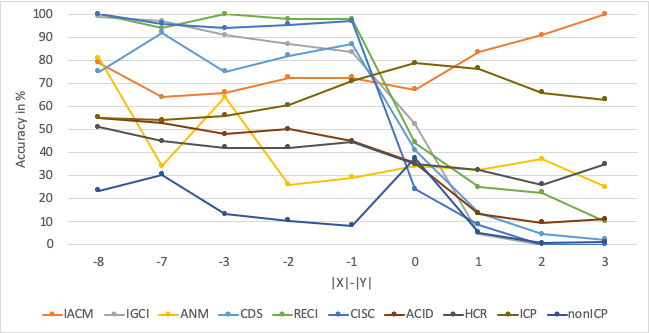
\includegraphics[scale=2.5]{result_linear_discrete.png}
        \caption{Averaged accuracy of correct inferred causal direction for linear synthetic data relative to the difference in alphabet size $|\kX| - |\kY|$ for small range sizes. }
        \label{fig:discrete_linear}
 \end{minipage}
  \end{figure}
  
Figure \ref{fig:discrete_linear} shows the averaged accuracy of correct inferred causal direction for each method we took into account relative to the difference in alphabet size $|\kX| - |\kY|$. Our method performs substantially better for non-negative differences than all alternative approaches except for ICP. A similar picture can be seen in Figure \ref{fig:discrete_nonlinear} where the averaged accuracy is shown for nonlinear synthetic data. Therefore, it seems that our method is better suited for situations were the alphabet size of the cause is greater or equal to the alphabet size of the effect.
 
\begin{figure}[h]
\begin{minipage}[c]{\textwidth}
\centering
         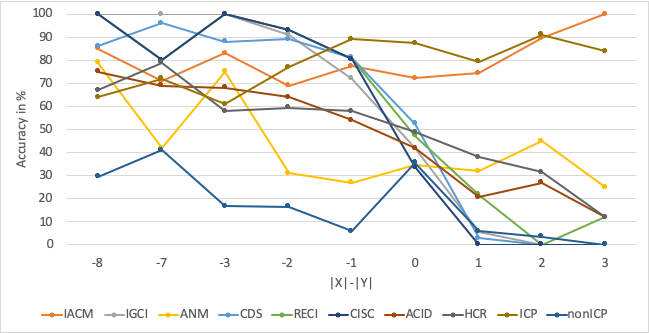
\includegraphics[scale=2.5]{result_nonlin_discrete.png}
        \caption{Averaged accuracy of correct inferred causal direction for nonlinear synthetic data relative to the difference in alphabet size $|\kX| - |\kY|$ for small range sizes. }
        \label{fig:discrete_nonlinear}
 \end{minipage}
\end{figure}

\subsection{Real-World Data}

As a benchmark set that consists of real-world data, we use a database of continuous cause-effect pairs that consists of manual labeled cause-effect pairs (CEP) from different contexts \cite{MPJZS16, DG19}. For all these pairs the ground truth is known and it is assumed that the pairs are not influenced by a confounder. As real-world discrete data sets we use anonymous discrete cause-effect pairs were food intolerances causes health issues (Food)\footnote{This dataset given as discrete timeseries data has been provided by the author and the causal direction has been independendly confirmed by medical tests.}, the Pittsburgh bridges dataset (Bridge) from \cite{DG19} as it has been used in \cite{CQZZH18}, and the Abalone dataset (Abalone) from the UCI Machine Learning Repository \cite{DG19}.

\begin{figure}[htb]
\begin{minipage}{\linewidth}
      \begin{minipage}{0.48\linewidth}
	      \centering
		  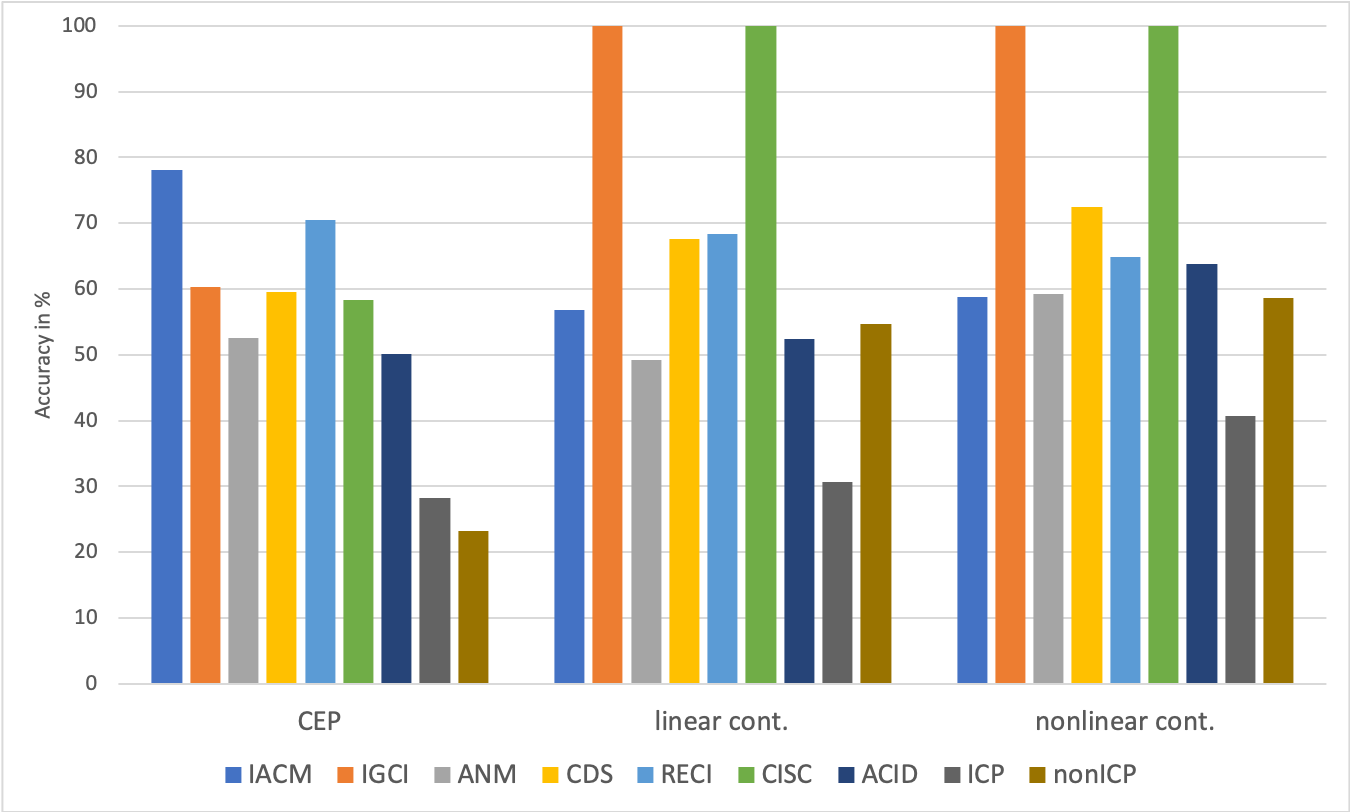
\includegraphics[scale=0.3]{results_cont_data.png}
           \subcaption{Accuracies of synthetic linear and nonlinear continuous data and of continuous real-world data (CEP).}
      \end{minipage}
      \hfill
      \begin{minipage}{0.48\linewidth}
	      \centering
  		  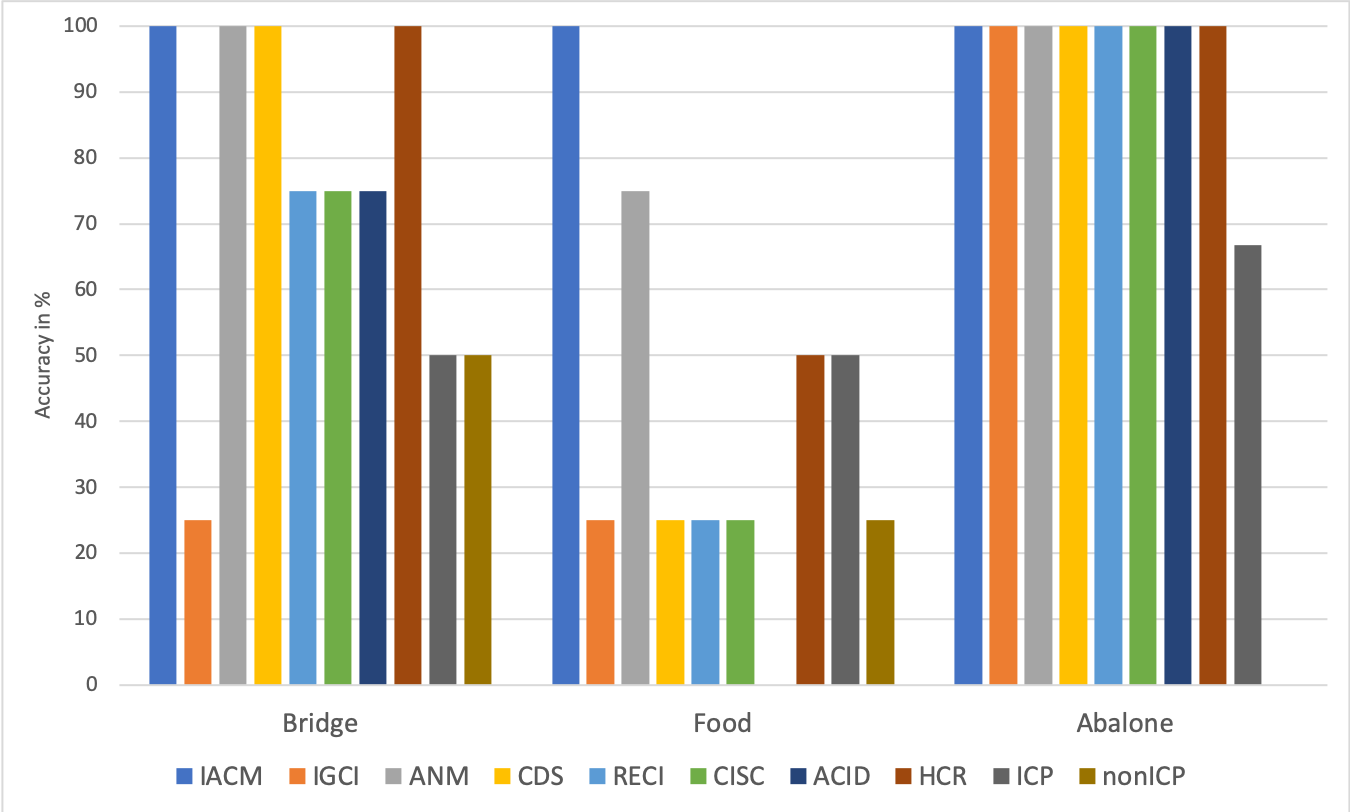
\includegraphics[scale=0.3]{result_real_discrete.png}
           \subcaption{Accuracies of different discrete real-world data sets.}
      \end{minipage}
       \caption{Accuracies of correct inferred causal directions for continuous and discrete data.}
       \label{fig.real_world_results}
  \end{minipage}
\end{figure}

In Figure \ref{fig.real_world_results} (a) we see that our method performs well for synthetic linear and nonlinear continuous data. For the CEP data set it outperforms all other methods. Also for discrete real-world data we can see in Figure \ref{fig.real_world_results} (b) that our methods successfully can recover all causal directions and can keep pace with state of the art methods.

\section{Discussion} \label{sec.discussion}

In this paper we proposed a way how empirical distributions that come from observations and experiments can be approximated to ones that follow the restrictions enforced by an assumed causal model. This approximated distribution can then be used to calculate probabilities of causation and together with the approximation error this leads to a new causal discovery method. In our experiments, we could confirm that our approach can compete with the current state of the art methods even on real-world datasets (continuous and discrete) and without the explicit knowledge of experimental data. Especially, for the discrete setting in which the alphabet size of the cause is greater or equal than the alphabet size of the effect our method has advantages compared to other approaches. ICP was the only method that performed better for synthetic data sets. However, for real-world data sets ICP seems too conservative and IACM was more reliable there. With a sophisticated preprocessing we also succeeded to apply that to the continuous setting with small $b_x$ and $b_y$. Therefore, it seems that in many cases we can encode the essential cause-effect information with much less information than we might have available in the data. This is interesting by itself and could serve as a base for future research.

\section*{Broader Impact}

The work in this paper could help to avoid unethical experiments.

\bibliographystyle{myamsalpha}
\bibliography{mrabbrev, references}

\end{document}
